% Options for packages loaded elsewhere
\PassOptionsToPackage{unicode}{hyperref}
\PassOptionsToPackage{hyphens}{url}
%
\documentclass[
]{article}
\usepackage{lmodern}
\usepackage{amssymb,amsmath}
\usepackage{ifxetex,ifluatex}
\ifnum 0\ifxetex 1\fi\ifluatex 1\fi=0 % if pdftex
  \usepackage[T1]{fontenc}
  \usepackage[utf8]{inputenc}
  \usepackage{textcomp} % provide euro and other symbols
\else % if luatex or xetex
  \usepackage{unicode-math}
  \defaultfontfeatures{Scale=MatchLowercase}
  \defaultfontfeatures[\rmfamily]{Ligatures=TeX,Scale=1}
\fi
% Use upquote if available, for straight quotes in verbatim environments
\IfFileExists{upquote.sty}{\usepackage{upquote}}{}
\IfFileExists{microtype.sty}{% use microtype if available
  \usepackage[]{microtype}
  \UseMicrotypeSet[protrusion]{basicmath} % disable protrusion for tt fonts
}{}
\makeatletter
\@ifundefined{KOMAClassName}{% if non-KOMA class
  \IfFileExists{parskip.sty}{%
    \usepackage{parskip}
  }{% else
    \setlength{\parindent}{0pt}
    \setlength{\parskip}{6pt plus 2pt minus 1pt}}
}{% if KOMA class
  \KOMAoptions{parskip=half}}
\makeatother
\usepackage{xcolor}
\IfFileExists{xurl.sty}{\usepackage{xurl}}{} % add URL line breaks if available
\IfFileExists{bookmark.sty}{\usepackage{bookmark}}{\usepackage{hyperref}}
\hypersetup{
  pdftitle={Scoring Matters: A Reproducible NEDC Evaluation of SeizureTransformer on TUSZ},
  pdfauthor={John H. Jung, MD, MS • Independent Researcher • jj@novamindnyc.com},
  hidelinks,
  pdfcreator={LaTeX via pandoc}}
\urlstyle{same} % disable monospaced font for URLs
\usepackage{color}
\usepackage{fancyvrb}
\newcommand{\VerbBar}{|}
\newcommand{\VERB}{\Verb[commandchars=\\\{\}]}
\DefineVerbatimEnvironment{Highlighting}{Verbatim}{commandchars=\\\{\}}
% Add ',fontsize=\small' for more characters per line
\newenvironment{Shaded}{}{}
\newcommand{\AlertTok}[1]{\textcolor[rgb]{1.00,0.00,0.00}{\textbf{#1}}}
\newcommand{\AnnotationTok}[1]{\textcolor[rgb]{0.38,0.63,0.69}{\textbf{\textit{#1}}}}
\newcommand{\AttributeTok}[1]{\textcolor[rgb]{0.49,0.56,0.16}{#1}}
\newcommand{\BaseNTok}[1]{\textcolor[rgb]{0.25,0.63,0.44}{#1}}
\newcommand{\BuiltInTok}[1]{#1}
\newcommand{\CharTok}[1]{\textcolor[rgb]{0.25,0.44,0.63}{#1}}
\newcommand{\CommentTok}[1]{\textcolor[rgb]{0.38,0.63,0.69}{\textit{#1}}}
\newcommand{\CommentVarTok}[1]{\textcolor[rgb]{0.38,0.63,0.69}{\textbf{\textit{#1}}}}
\newcommand{\ConstantTok}[1]{\textcolor[rgb]{0.53,0.00,0.00}{#1}}
\newcommand{\ControlFlowTok}[1]{\textcolor[rgb]{0.00,0.44,0.13}{\textbf{#1}}}
\newcommand{\DataTypeTok}[1]{\textcolor[rgb]{0.56,0.13,0.00}{#1}}
\newcommand{\DecValTok}[1]{\textcolor[rgb]{0.25,0.63,0.44}{#1}}
\newcommand{\DocumentationTok}[1]{\textcolor[rgb]{0.73,0.13,0.13}{\textit{#1}}}
\newcommand{\ErrorTok}[1]{\textcolor[rgb]{1.00,0.00,0.00}{\textbf{#1}}}
\newcommand{\ExtensionTok}[1]{#1}
\newcommand{\FloatTok}[1]{\textcolor[rgb]{0.25,0.63,0.44}{#1}}
\newcommand{\FunctionTok}[1]{\textcolor[rgb]{0.02,0.16,0.49}{#1}}
\newcommand{\ImportTok}[1]{#1}
\newcommand{\InformationTok}[1]{\textcolor[rgb]{0.38,0.63,0.69}{\textbf{\textit{#1}}}}
\newcommand{\KeywordTok}[1]{\textcolor[rgb]{0.00,0.44,0.13}{\textbf{#1}}}
\newcommand{\NormalTok}[1]{#1}
\newcommand{\OperatorTok}[1]{\textcolor[rgb]{0.40,0.40,0.40}{#1}}
\newcommand{\OtherTok}[1]{\textcolor[rgb]{0.00,0.44,0.13}{#1}}
\newcommand{\PreprocessorTok}[1]{\textcolor[rgb]{0.74,0.48,0.00}{#1}}
\newcommand{\RegionMarkerTok}[1]{#1}
\newcommand{\SpecialCharTok}[1]{\textcolor[rgb]{0.25,0.44,0.63}{#1}}
\newcommand{\SpecialStringTok}[1]{\textcolor[rgb]{0.73,0.40,0.53}{#1}}
\newcommand{\StringTok}[1]{\textcolor[rgb]{0.25,0.44,0.63}{#1}}
\newcommand{\VariableTok}[1]{\textcolor[rgb]{0.10,0.09,0.49}{#1}}
\newcommand{\VerbatimStringTok}[1]{\textcolor[rgb]{0.25,0.44,0.63}{#1}}
\newcommand{\WarningTok}[1]{\textcolor[rgb]{0.38,0.63,0.69}{\textbf{\textit{#1}}}}
\usepackage{longtable,booktabs}
% Correct order of tables after \paragraph or \subparagraph
\usepackage{etoolbox}
\makeatletter
\patchcmd\longtable{\par}{\if@noskipsec\mbox{}\fi\par}{}{}
\makeatother
% Allow footnotes in longtable head/foot
\IfFileExists{footnotehyper.sty}{\usepackage{footnotehyper}}{\usepackage{footnote}}
\makesavenoteenv{longtable}
\usepackage{graphicx}
\makeatletter
\def\maxwidth{\ifdim\Gin@nat@width>\linewidth\linewidth\else\Gin@nat@width\fi}
\def\maxheight{\ifdim\Gin@nat@height>\textheight\textheight\else\Gin@nat@height\fi}
\makeatother
% Scale images if necessary, so that they will not overflow the page
% margins by default, and it is still possible to overwrite the defaults
% using explicit options in \includegraphics[width, height, ...]{}
\setkeys{Gin}{width=\maxwidth,height=\maxheight,keepaspectratio}
% Set default figure placement to htbp
\makeatletter
\def\fps@figure{htbp}
\makeatother
\setlength{\emergencystretch}{3em} % prevent overfull lines
\providecommand{\tightlist}{%
  \setlength{\itemsep}{0pt}\setlength{\parskip}{0pt}}
\setcounter{secnumdepth}{-\maxdimen} % remove section numbering
% Extra header for arXiv build: float control + graphics path
\usepackage{caption}
\usepackage{ragged2e}
% Tighter, cleaner figure captions: justified text, colon after label, minimal vertical gaps
\captionsetup[figure]{%
  font=small,
  labelfont=bf,
  labelsep=colon,
  format=plain,
  justification=justified,
  singlelinecheck=false,
  width=0.85\linewidth,
  skip=1.5pt,
  belowskip=1.5pt
}

% Keep figures near their sections
\usepackage[section]{placeins}

% Improve float behavior and spacing
\makeatletter
\def\fps@figure{!htbp}
\makeatother
\renewcommand{\topfraction}{0.92}
\renewcommand{\bottomfraction}{0.85}
\renewcommand{\textfraction}{0.06}
\renewcommand{\floatpagefraction}{0.92}
% Tighter spacing around floats
\setlength{\textfloatsep}{6pt plus 2pt minus 2pt}
\setlength{\intextsep}{6pt plus 2pt minus 2pt}
\setlength{\floatsep}{6pt plus 2pt minus 2pt}

% Look for figures in both the current dir and the original figures path
\usepackage{graphicx}
\graphicspath{{.}{figures/output/arxiv/}}

% Map common Unicode characters for pdflatex compatibility (not needed on XeLaTeX/LuaLaTeX)
\usepackage{ifxetex,ifluatex}
\ifnum 0\ifxetex 1\fi\ifluatex 1\fi=0
  \DeclareUnicodeCharacter{2212}{-}   % minus sign
  \DeclareUnicodeCharacter{2013}{--}  % en dash
  \DeclareUnicodeCharacter{2014}{---} % em dash
\fi

\title{Scoring Matters: A Reproducible NEDC Evaluation of
SeizureTransformer on TUSZ}
\usepackage{etoolbox}
\makeatletter
\providecommand{\subtitle}[1]{% add subtitle to \maketitle
  \apptocmd{\@title}{\par {\large #1 \par}}{}{}
}
\makeatother
\subtitle{A 27--137× gap between claims and reproducible evaluation on
TUSZ}
\author{John H. Jung, MD, MS • Independent Researcher •
jj@novamindnyc.com}
\date{September 2025}

\begin{document}
\maketitle

\hypertarget{abstract}{%
\subsection{Abstract}\label{abstract}}

Claims about deep learning model performance in seizure detection are
difficult to verify without standardized evaluation protocols. We report
the first evaluation of SeizureTransformer on the Temple University
Hospital EEG Seizure Corpus (TUSZ) {[}2{]} using the Neural Engineering
Data Consortium (NEDC) v6.0.0 scoring tools {[}3{]}---the same
evaluation framework used in peer-reviewed literature for two decades.
Despite being trained on TUSZ, SeizureTransformer has never been
evaluated on it using Temple's official scoring software. We find a
27-137x gap between the \textasciitilde1 false alarm per 24 hours
reported on the EpilepsyBench Dianalund dataset {[}1{]} and clinical
reality.

We evaluate the authors' pretrained model on TUSZ v2.0.3's held-out set
(865 files, 127.7 hours) and assess identical predictions with three
scoring methodologies. With NEDC OVERLAP {[}3{]}, the model produces
26.89 FA/24h; with SzCORE Event {[}4{]}, 8.59 FA/24h
(\textasciitilde=3.1x lower due solely to scoring tolerances); with NEDC
TAES {[}5{]}, 136.73 FA/24h.

When tuned toward deployment goals, the model cannot meet clinical
thresholds with NEDC scoring: targeting 10 FA/24h achieves only 33.90\%
sensitivity, far below the 75\% sensitivity goal for clinical systems
{[}13{]}. Acceptable false-alarm rates occur only under SzCORE Event's
permissive tolerances {[}4{]}.

We contribute a reproducible NEDC evaluation pipeline, operating points
tailored to clinical targets, and quantitative evidence that scoring
choice alone drives multi-fold differences. Dataset-matched,
clinician-aligned evaluation is essential for credible seizure-detection
claims.

\hypertarget{introduction}{%
\section{Introduction}\label{introduction}}

The evaluation of seizure detection algorithms suffers from a
fundamental reproducibility crisis. Published models report dramatically
different performance metrics while claiming state-of-the-art results,
yet these claims often cannot be verified due to proprietary datasets,
missing evaluation code, or ambiguous scoring definitions. This opacity
particularly affects deep learning approaches, where complex
architectures and extensive hyperparameter spaces compound the
verification challenge.

SeizureTransformer {[}1{]} exemplifies this problem. The model reports
37\% sensitivity at 1.0 FA/24h on a proprietary Danish dataset
(Dianalund), with no public evaluation possible. While the authors
released model weights---a commendable step toward reproducibility---the
absence of standardized evaluation on public datasets leaves critical
questions unanswered about real-world performance. When we evaluated
this same model on the dataset it was trained on, using the official
scoring software designed for that dataset, we discovered false alarm
rates 27 to 137 times higher than claimed, depending on the scoring
methodology employed.

SeizureTransformer represents a significant architectural advance in
seizure detection, combining U-Net's proven biomedical segmentation
capabilities with Transformer self-attention mechanisms to capture both
local and global EEG patterns. The model was trained on a subset of the
Temple University Hospital Seizure (TUSZ) dataset (v2.0.3;
\textasciitilde910 hours) together with the Siena Scalp EEG Database
(\textasciitilde128 hours) {[}9{]}. TUSZ itself is the largest publicly
available seizure corpus, but the model's training used a subset as
reported by the authors. Its victory in EpilepsyBench 2025, achieving
37\% sensitivity at 1 FA/24h on the Dianalund dataset, established it as
the state-of-the-art in automated seizure detection. The authors openly
shared their pretrained weights, enabling reproducible research and
clinical validation.

Despite this success, a critical evaluation gap exists. While
SeizureTransformer was trained on TUSZ's training set, no published
evaluation exists using TUSZ's carefully designed, patient-disjoint
held-out evaluation set. This 127.7-hour test set, containing 865 files
from 43 patients with 469 seizures, was specifically created to enable
valid performance assessment. Moreover, Temple University's Neural
Engineering Data Consortium (NEDC) developed scoring software explicitly
to match TUSZ's annotation philosophy, ensuring consistent evaluation
standards. The absence of TUSZ evaluation is not unique to
SeizureTransformer---it reflects a broader pattern where models trained
on datasets are evaluated elsewhere, with results reported using varying
scoring methodologies.

The choice of scoring methodology profoundly impacts reported
performance. The seizure detection community employs multiple evaluation
standards, each serving different purposes. NEDC implements strict
temporal precision matching Temple's conservative annotation guidelines.
In contrast, SzCORE Event---the EpilepsyBench standard---adds 30-second
pre-ictal and 60-second post-ictal tolerances around ground truth
events, designed to reward clinically useful early warnings. These
philosophical differences are not matters of right or wrong but reflect
different priorities: research precision versus clinical utility.
However, when the same predictions can yield anywhere from 8.59 to
136.73 false alarms per 24 hours purely based on scoring choice, the
lack of standardized reporting becomes problematic.

We present, to our knowledge, the first evaluation of SeizureTransformer
on TUSZ's held-out test set using Temple's NEDC v6.0.0 scoring software.
Our systematic comparison evaluates identical model predictions using
three scoring methodologies: NEDC TAES (time-aligned event scoring),
NEDC OVERLAP (binary any-overlap), and SzCORE Event. At the paper's
default parameters (threshold=0.8, kernel=5, duration=2.0s), we observe
45.63\% sensitivity at 26.89 FA/24h with NEDC OVERLAP---a 27-fold
increase from the Dianalund benchmark claim. The same predictions yield
136.73 FA/24h with NEDC TAES (137-fold increase) and 8.59 FA/24h with
SzCORE Event. This 3.1-fold difference between NEDC OVERLAP and SzCORE
Event stems entirely from scoring methodology, independent of model
architecture or parameters.

\begin{figure}
\hypertarget{fig:performance-gap}{%
\centering
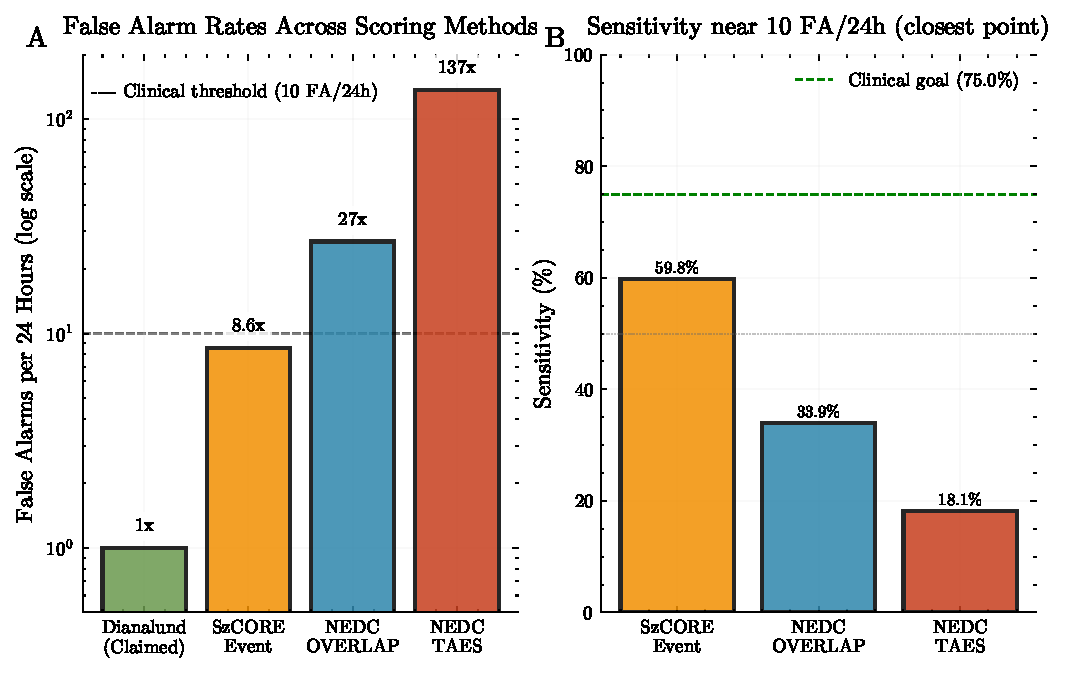
\includegraphics[width=0.75\textwidth,height=\textheight]{figures/output/arxiv/FIGURE_1_performance_gap.pdf}
\caption{Performance gap visualization showing the 27--137× difference
between claimed and measured false alarm rates. Panel A shows false
alarm rates on a logarithmic scale, comparing Dianalund's claimed
performance (1 FA/24h) against our TUSZ evaluation using different
scoring methods. Panel B displays sensitivity near 10 FA/24h using each
scorer's closest available operating point (no interpolation). SzCORE
Event uses any-overlap with clinical tolerances (−30 s/+60 s; merge
\textless90 s, split \textgreater5 min).}\label{fig:performance-gap}
}
\end{figure}

Our contributions extend beyond revealing performance gaps. We provide:
(1) a reproducible NEDC v6.0.0 evaluation pipeline for TUSZ, bridging
the research-to-clinic evaluation gap {[}3{]}; (2) comprehensive
operating points for clinical deployment, including evaluation at a
clinically-motivated threshold of \textless=10 FA/24h; (3) quantitative
evidence that scoring methodology alone can account for multi-fold
performance differences, highlighting the critical need for transparent
reporting; and (4) open-source infrastructure enabling the community to
replicate and extend our evaluation framework. When optimizing for the
10 FA/24h threshold, SeizureTransformer achieves only 33.90\%
sensitivity with NEDC OVERLAP, falling far short of the 75\% sensitivity
goal for clinical systems {[}13{]}.

The remainder of this paper is organized as follows. Section 2 provides
background and related work on TUSZ, NEDC, and scoring methodologies.
Section 3 details our evaluation methodology, including data
preparation, model inference, and multi-scorer validation. Section 4
presents comprehensive results across multiple operating points and
scoring methods. Section 5 discusses implications for clinical
deployment, the need for standardized evaluation, and limitations of
current benchmarking practices. Section 6 concludes. Section 7 outlines
reproducibility resources and exact rerun procedures.

\hypertarget{background-and-related-work}{%
\section{Background and Related
Work}\label{background-and-related-work}}

The Temple University Hospital Seizure Corpus (TUSZ) is the largest
publicly available seizure dataset {[}2{]}. Critically, TUSZ implements
patient-disjoint train/dev/eval splits---no patient appears in multiple
splits---preventing data leakage and enabling valid generalization
assessment. The evaluation set contains 865 EDF files totaling 127.7
hours from 43 patients with 469 seizures, specifically reserved for
final held-out testing {[}2{]}. This careful split design follows
machine learning best practices often violated in medical AI
applications. The annotations, performed by highly trained
undergraduates and validated against board-certified neurologists
{[}2{]}, follow conservative clinical guidelines requiring clear
electrographic seizures with definite evolution and temporal precision
in marking onset and offset.

Alongside TUSZ, Temple University's Neural Engineering Data Consortium
(NEDC) developed the scoring software suite, creating a matched
evaluation ecosystem {[}3{]}. NEDC v6.0.0 provides the definitive
scoring implementation for TUSZ evaluation {[}3{]}. This matched pairing
is no coincidence---the same research group created both the dataset and
its evaluation tools, ensuring consistency between annotation philosophy
and scoring methodology. NEDC implements multiple scoring modes, with
OVERLAP (any-overlap binary scoring) serving as the commonly reported
evaluation mode for TUSZ. The software is widely used in the literature
and serves as a reference implementation for seizure detection
evaluation {[}3{]}.

The choice of scoring methodology profoundly impacts reported
performance, as different methods serve distinct clinical and research
priorities. Time-Aligned Event Scoring (TAES), proposed by Shah et
al.~{[}5{]}, represents the strictest evaluation standard, computing
partial credit based on temporal overlap percentage---a 60-second
seizure with 45 seconds correctly detected receives 0.75 true positive
credit {[}5{]}. TAES emphasizes temporal precision, making it ideal for
algorithm development and research applications where exact timing
matters. In contrast, OVERLAP scoring, which NEDC implements as a
primary mode, treats any temporal overlap between prediction and ground
truth as a full true positive {[}3{]}. Shah et al.~{[}5{]} note that
``OVLP is considered a very permissive way of scoring since any amount
of overlap between a reference and hypothesis event constitutes a true
positive,'' yet this binary approach has become a de facto standard for
TUSZ reporting, balancing clinical relevance with research needs.

At the most permissive end of the spectrum, SzCORE Event {[}4{]} extends
any-overlap scoring with clinical tolerances designed for real-world
deployment. The system adds 30-second pre-ictal and 60-second post-ictal
windows around each ground truth event {[}4{]}, recognizing that early
warnings before seizure onset provide clinical value and that EEG
patterns normalize gradually after seizure termination. Additionally,
SzCORE Event merges predictions separated by less than 90 seconds into
single events, substantially reducing alarm fatigue in clinical settings
{[}4{]}. These modifications, while clinically motivated, can
substantially reduce reported false alarm rates compared to stricter
scoring methods---as we demonstrate in our results, observing a 3.1x
reduction between NEDC OVERLAP and SzCORE Event. Importantly, these
different approaches represent not right or wrong methods but rather
different valid perspectives on what constitutes meaningful seizure
detection---research precision versus clinical utility versus deployment
practicality.

Scoring paradigms broadly fall into event-based (e.g., OVERLAP, TAES,
SzCORE Event) and sample-based (epoch) methods. Event-based evaluation
aligns with clinical interpretation of seizures as discrete neurological
events. Sample-based methods compare 1 Hz labels and can conflate
non-seizure accuracy with seizure detection utility; therefore, all
results in this work use event-based metrics. See Methods for precise
definitions and the rationale for this choice.

SeizureTransformer {[}10{]} exemplifies both the advances and evaluation
gaps in modern seizure detection. The architecture combines U-Net's
biomedical segmentation capabilities with Transformer self-attention to
capture local and global EEG patterns {[}10{]}. Trained on a subset of
TUSZ v2.0.3 (\textasciitilde910 hours) {[}2{]} plus the Siena Scalp EEG
Database (128 hours) {[}9{]}, the model processes 19-channel EEG at 256
Hz through 60-second windows {[}10{]}. With publicly available
pretrained weights (we measured approximately 41 million parameters,
\textasciitilde168 MB file size), SeizureTransformer won the
EpilepsyBench Challenge, achieving 37\% sensitivity at 1 false alarm per
24 hours on the Dianalund dataset {[}10{]}---a Danish long-term
monitoring corpus distinct from its training data. The authors' decision
to openly share their weights enables reproducible evaluation, a
practice we build on here {[}10{]}.

Despite training on TUSZ, SeizureTransformer has never been evaluated on
TUSZ's held-out evaluation set using Temple's official scoring software
{[}3{]}. EpilepsyBench marks TUSZ results with a train emoji
({[}train{]}) {[}10{]}, indicating the model was trained on this dataset
and therefore showing no evaluation metrics. While this conservative
approach prevents overfitting claims, it overlooks the careful
patient-disjoint split design that specifically enables valid held-out
evaluation {[}2{]}. This represents a broader pattern in the field:
models are trained on Dataset X, evaluated on Dataset Y with favorable
scoring, generalization is claimed, yet performance on X's properly
designed evaluation set remains unknown {[}11{]}. The uniform
application of SzCORE Event scoring across all EpilepsyBench datasets,
while ensuring consistency, obscures dataset-specific performance that
would be revealed by matched evaluation tools {[}10{]}.

The clinical deployment of seizure detection systems requires meeting
stringent performance thresholds. Clinical goals typically target 75\%
sensitivity or higher {[}13{]}, while human reviewers achieve
approximately 1 false alarm per 24 hours {[}13{]}. These requirements
reflect the reality of clinical workflows where excessive false alarms
lead to alarm fatigue and system abandonment. However, whether a system
meets these thresholds depends critically on the evaluation methodology
employed. Previous work has highlighted challenges in cross-dataset
generalization {[}2{]}, the need for standardized evaluation metrics
{[}4{]}, and broader reproducibility issues in medical AI {[}11{]}. Our
work addresses these challenges by performing the missing evaluation:
testing SeizureTransformer on TUSZ's held-out set using multiple scoring
methodologies, revealing how evaluation choices fundamentally shape
performance claims in seizure detection systems.

\hypertarget{methods}{%
\section{Methods}\label{methods}}

We evaluated SeizureTransformer on the TUSZ v2.0.3 held-out test set
using the authors' pretrained weights without modification {[}1{]}. Our
evaluation employed three distinct scoring methodologies on identical
model predictions to quantify the impact of evaluation standards on
reported performance.

\hypertarget{dataset}{%
\subsection{Dataset}\label{dataset}}

We used the Temple University Hospital Seizure Corpus (TUSZ) v2.0.3,
focusing on its carefully designed evaluation split {[}2{]}. The eval
set contains 865 EDF files totaling 127.7 hours from 43 patients with
469 expert-annotated seizures {[}2{]}. Critically, this set is
patient-disjoint from the training and development splits, ensuring no
data leakage and enabling valid generalization assessment {[}2{]}. We
achieved 100\% file coverage, with one file requiring automated header
repair using pyEDFlib's repair functionality on a temporary copy
{[}12{]}.

The development set, containing 1,832 files (435.5 hours) from 53
distinct patients with 1,075 seizures, was used exclusively for
post-processing parameter optimization. This maintains the integrity of
the held-out evaluation while allowing systematic exploration of
clinical operating points.

\hypertarget{model-and-inference-pipeline}{%
\subsection{Model and Inference
Pipeline}\label{model-and-inference-pipeline}}

We employed the authors' publicly available pretrained
SeizureTransformer weights (\textasciitilde=168 MB) without any
modifications, retraining, or fine-tuning {[}1{]}. The model expects
19-channel unipolar montage EEG data sampled at 256 Hz, processing
60-second windows (15,360 samples per channel) through its
U-Net-Transformer architecture {[}1{]}.

Our preprocessing pipeline, implemented as a wrapper around the original
wu\_2025 code, follows the paper's specifications {[}1{]}. For each EDF
file, we: (1) load the data with unipolar montage enforcement and
normalized channel aliases; (2) apply per-channel z-score normalization
across the full recording; (3) resample to 256 Hz if necessary; (4)
apply a 0.5-120 Hz bandpass filter (3rd-order Butterworth); and (5)
apply notch filters at 1 Hz and 60 Hz (Q=30) as specified in the
original paper and implementation {[}1{]}.

The model processes 60-second non-overlapping windows, outputting
per-sample seizure probabilities at 256 Hz. Post-processing applies
three sequential operations using configurable parameters: (1) threshold
the probability values to create a binary mask; (2) apply morphological
opening and closing operations with a specified kernel size; and (3)
remove events shorter than a minimum duration. The paper's default
configuration uses threshold theta=0.8, kernel size k=5 samples, and
minimum duration d=2.0 seconds {[}1{]}.

\hypertarget{scoring-methodologies}{%
\subsection{Scoring Methodologies}\label{scoring-methodologies}}

We evaluated identical model predictions using three scoring
methodologies, each representing different clinical and research
priorities:

\textbf{NEDC TAES (Time-Aligned Event Scoring)} computes partial credit
based on temporal overlap between predictions and ground truth {[}5{]}.
If a 60-second reference seizure has 45 seconds correctly detected, TAES
awards 0.75 true positive credit {[}5{]}. This methodology emphasizes
temporal precision, making it the strictest evaluation standard.

\textbf{NEDC OVERLAP} implements Temple's binary any-overlap scoring
within the NEDC v6.0.0 framework {[}3{]}. Any temporal overlap between
prediction and reference, regardless of duration, counts as a full true
positive. This represents the commonly reported mode for TUSZ
evaluation, matching the dataset's annotation philosophy {[}3{]}.

\textbf{SzCORE Event (Any-Overlap + tolerances)} extends binary scoring
with clinical tolerances: 30-second pre-ictal and 60-second post-ictal
windows around each reference event, plus merging of predictions
separated by less than 90 seconds {[}4{]}. These modifications, designed
for clinical deployment scenarios where early warnings and reduced alarm
fatigue are prioritized, substantially reduce reported false alarm rates
{[}4{]}.

All scoring implementations process the same binary prediction masks,
ensuring that performance differences stem solely from scoring
philosophy rather than model behavior.

\hypertarget{choice-of-event-based-metrics}{%
\subsubsection{Choice of Event-Based
Metrics}\label{choice-of-event-based-metrics}}

We report only event-based metrics (NEDC OVERLAP, NEDC TAES, SzCORE
Event) because clinical evaluation focuses on detecting discrete seizure
events. Sample-based (epoch) methods (e.g., NEDC EPOCH; SzCORE
Sample-based) compare 1 Hz labels and can inflate scores by rewarding
long non-seizure periods, obscuring event detection quality. To avoid
this pitfall, all reported results are event-based. ``SzCORE Event''
denotes any-overlap with ±30 s/60 s tolerances and merge/split rules
(merge \textless90 s, split \textgreater5 min); we do not report SzCORE
Sample-based.

\begin{figure}
\hypertarget{fig:scoring-impact}{%
\centering
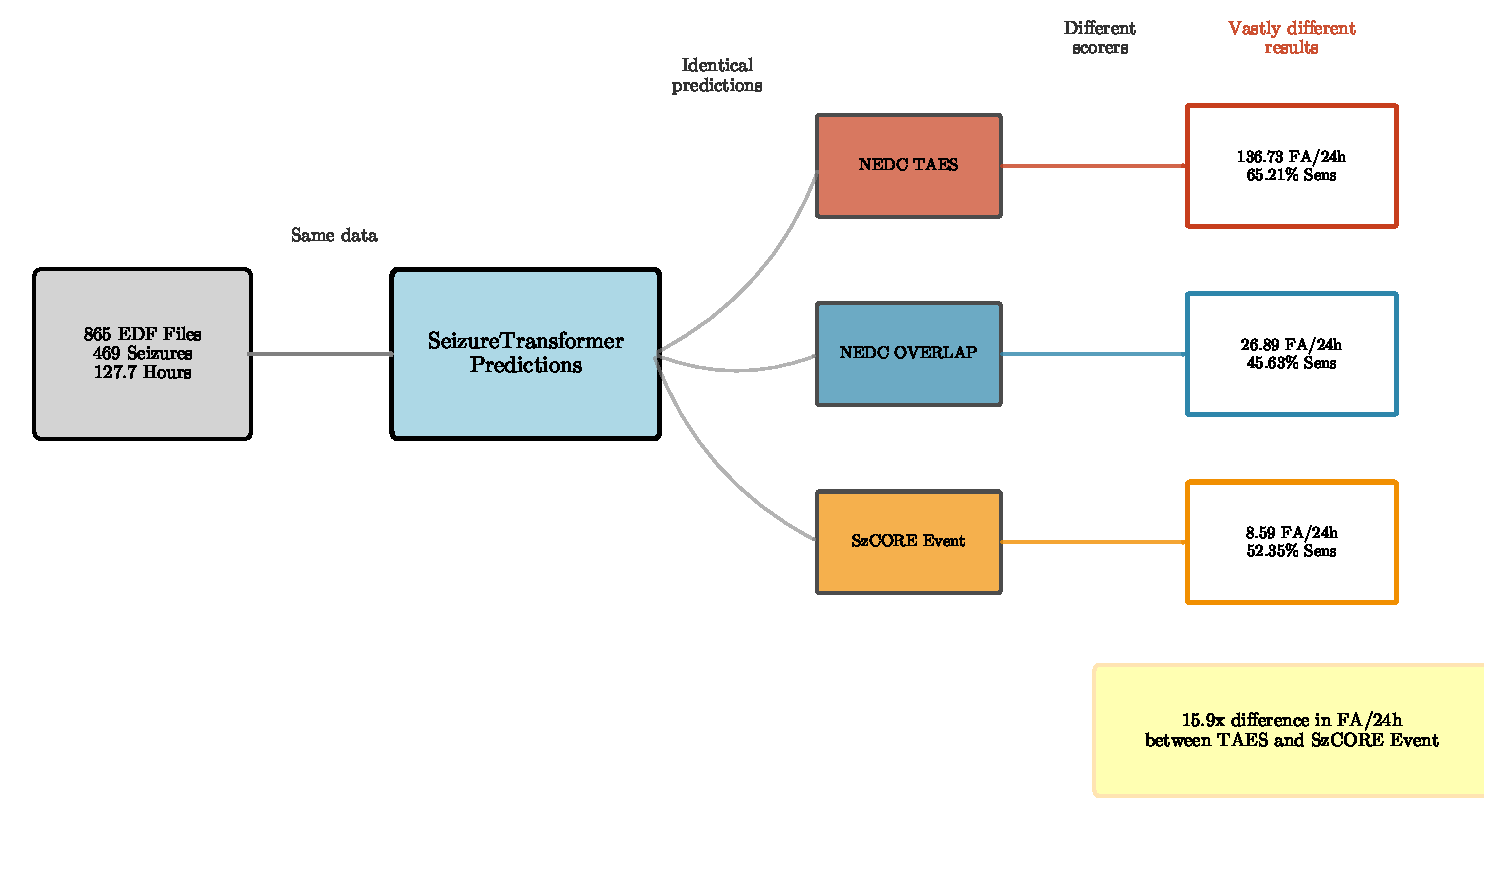
\includegraphics[width=0.7\textwidth,height=\textheight]{figures/output/arxiv/FIGURE_2_scoring_impact.pdf}
\caption{Impact of scoring methodology on reported performance. The same
SeizureTransformer predictions flow through different scoring pipelines,
yielding a 15.9x difference in false alarm rates between NEDC TAES and
SzCORE Event. This visualization demonstrates how evaluation standards,
not model improvements, can account for order-of-magnitude performance
variations.}\label{fig:scoring-impact}
}
\end{figure}

\hypertarget{parameter-optimization}{%
\subsection{Parameter Optimization}\label{parameter-optimization}}

We conducted systematic post-processing parameter optimization on the
TUSZ development set, targeting clinical deployment criteria of
\textless=10 false alarms per 24 hours while maximizing sensitivity. Our
grid search explored: thresholds theta in \{0.60, 0.65, 0.70, 0.75,
0.80, 0.85, 0.88, 0.90, 0.92, 0.95, 0.98\}, morphological kernel sizes k
in \{3, 5, 7, 9, 11, 13, 15\} samples, and minimum event durations d in
\{1.0, 1.5, 2.0, 2.5, 3.0, 3.5, 4.0, 4.5, 5.0, 6.0\} seconds.

For each configuration, we computed sensitivity and false alarm rates
using NEDC OVERLAP scoring, as this is the commonly reported mode for
TUSZ. From the resulting parameter space, we selected operating points
for comprehensive evaluation: (1) \textbf{Default} (theta=0.80, k=5,
d=2.0s) --- the paper's published configuration; (2) \textbf{Clinical 10
FA/24h target} (theta=0.88, k=5, d=3.0s) --- optimized to meet the
\textless=10 FA/24h constraint; and (3) \textbf{ICU-like 2.5 FA/24h
target} (theta=0.95, k=5, d=5.0s) --- a more conservative operating
point. We additionally report selected high-threshold points (e.g.,
theta=0.98) when illustrating the full trade-off curve.

\begin{figure}
\hypertarget{fig:parameter-heatmap}{%
\centering
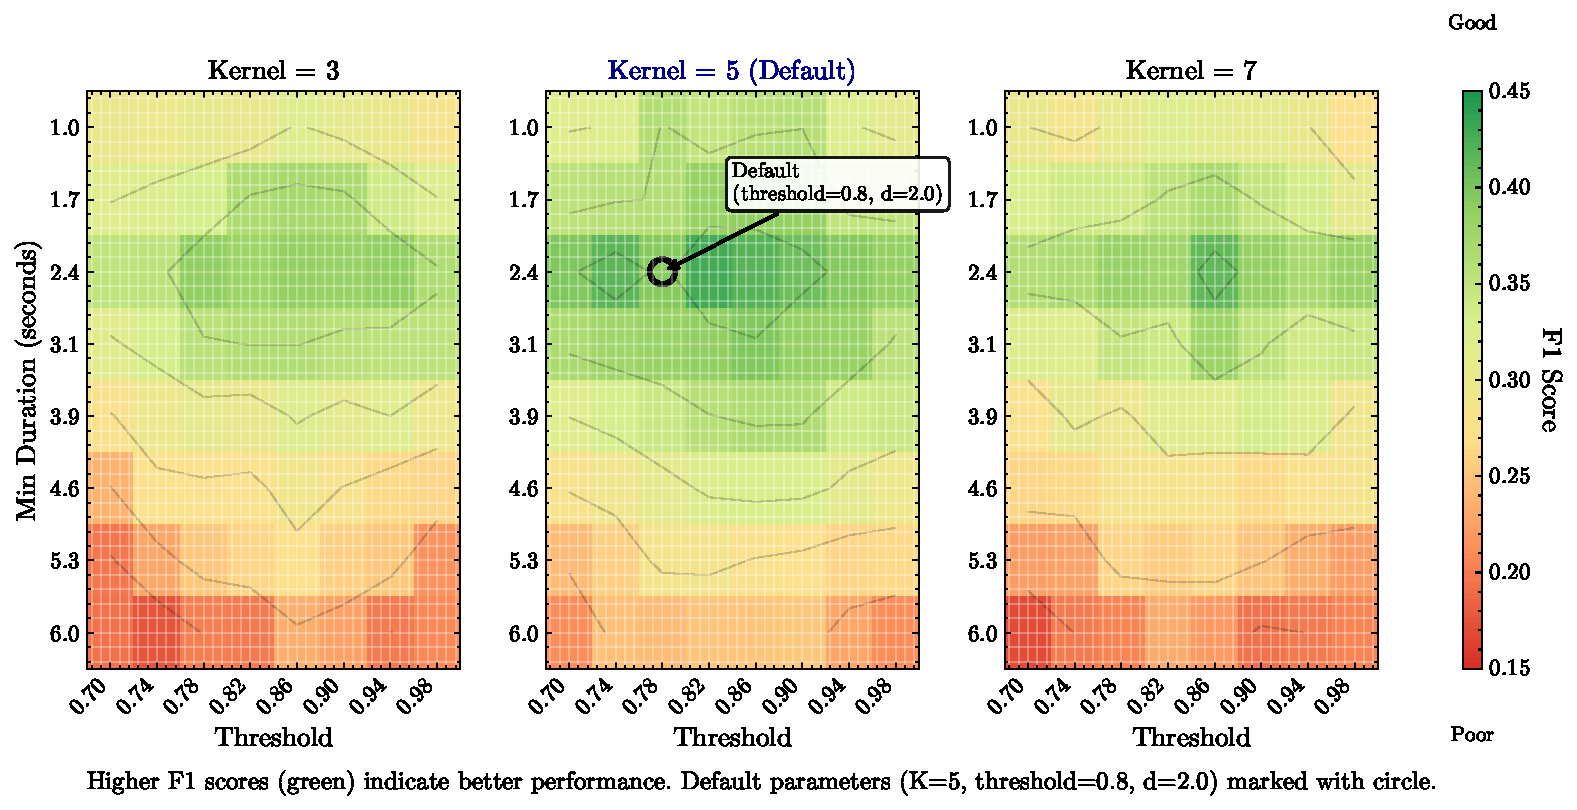
\includegraphics[width=0.88\textwidth,height=\textheight]{figures/output/arxiv/FIGURE_3_parameter_heatmap.pdf}
\caption{Parameter sensitivity analysis showing F1 scores across
threshold and minimum duration values for NEDC OVERLAP scoring. The
heatmaps reveal that optimal parameters vary by morphological kernel
size, with the paper's default (theta=0.8, d=2.0) marked. Higher
thresholds are required to achieve clinically acceptable false alarm
rates.}\label{fig:parameter-heatmap}
}
\end{figure}

\hypertarget{implementation-and-validation}{%
\subsection{Implementation and
Validation}\label{implementation-and-validation}}

Our evaluation pipeline integrates multiple software components to
ensure reproducibility and clinical validity. Model inference uses the
original wu\_2025 codebase with our preprocessing wrapper. Predictions
are converted to NEDC's CSV\_bi format, which requires specific
formatting: four decimal places for timestamps, ``TERM'' as the channel
identifier, and standardized header metadata including file duration.

We validated our implementation through consistency checks across tools
and confirmed that all 865 eval files were successfully processed (with
one automated header repair). Reported results use the official NEDC
scorers and SzCORE Event.

To enable full reproducibility, we provide our complete evaluation
codebase, including the preprocessing wrapper, scoring implementations,
and parameter optimization scripts. The pretrained SeizureTransformer
weights remain available from the authors' repository, and NEDC v6.0.0
can be obtained from Temple University.

\hypertarget{statistical-analysis}{%
\subsection{Statistical Analysis}\label{statistical-analysis}}

We report standard seizure detection metrics for each configuration and
scorer combination: sensitivity (seizure-level recall), false alarm rate
per 24 hours (computed from total recording duration), and F1 score. For
NEDC scorers, we report SEIZ-only FA/24h as the primary metric (Temple's
``Total FA'' is archived in summaries). For SzCORE Event, we follow its
event-based false positive definition. We also computed AUROC across
threshold values to assess overall discriminative capability independent
of operating point selection.

This comprehensive evaluation framework, combining the authors'
pretrained model with multiple scoring standards applied to a properly
held-out test set, reveals how methodological choices fundamentally
shape reported performance metrics in seizure detection systems.

\hypertarget{results}{%
\section{Results}\label{results}}

\hypertarget{evaluation-setup}{%
\subsection{Evaluation Setup}\label{evaluation-setup}}

We evaluated SeizureTransformer on TUSZ v2.0.3's held-out evaluation set
containing 865 EEG files (127.7 hours of recordings). Using the authors'
pretrained weights, we generated predictions and evaluated them using
three scoring methodologies: NEDC OVERLAP (Temple's official any-overlap
mode), NEDC TAES (time-aligned), and SzCORE Event (EpilepsyBench
standard).

\hypertarget{primary-results}{%
\subsection{Primary Results}\label{primary-results}}

\hypertarget{default-configuration-theta0.80-k5-d2.0}{%
\subsubsection{Default Configuration (theta=0.80, k=5,
d=2.0)}\label{default-configuration-theta0.80-k5-d2.0}}

At the paper's default parameters, we observed dramatic variation across
scoring methods. The same predictions yielded:

\begin{itemize}
\tightlist
\item
  \textbf{NEDC OVERLAP}: 45.63\% sensitivity, 26.89 FA/24h
\item
  \textbf{NEDC TAES}: 65.21\% sensitivity, 136.73 FA/24h
\item
  \textbf{SzCORE Event}: 52.35\% sensitivity, 8.59 FA/24h
\end{itemize}

This represents a \textbf{3.1x difference} in false alarm rates between
NEDC OVERLAP and SzCORE Event scoring on identical predictions. Compared
to the paper's reported \textasciitilde1 FA/24h on Dianalund, we observe
a \textbf{27-fold gap} with NEDC OVERLAP and a \textbf{137-fold gap}
with NEDC TAES.

\begin{longtable}[]{@{}lrrrr@{}}
\toprule
Scoring Method & Sensitivity (\%) & FA/24h & Multiplier vs Claimed & F1
Score\tabularnewline
\midrule
\endhead
\textbf{Dianalund (Claimed)} & 37.00 & 1.00 & 1x & 0.43*\tabularnewline
SzCORE Event & 52.35 & 8.59 & 9x & 0.485\tabularnewline
NEDC OVERLAP & 45.63 & 26.89 & \textbf{27x} & 0.414\tabularnewline
NEDC TAES & 65.21 & 136.73 & \textbf{137x} & 0.237\tabularnewline
\bottomrule
\end{longtable}

Table 1: Performance at default parameters (theta=0.80, k=5, d=2.0). *F1
from competition leaderboard.

\hypertarget{clinical-deployment-targets}{%
\subsubsection{Clinical Deployment
Targets}\label{clinical-deployment-targets}}

We optimized parameters on the development set to target clinical false
alarm thresholds:

\textbf{10 FA/24h Target (theta=0.88, k=5, d=3.0)}: - NEDC OVERLAP
achieved 33.90\% sensitivity at 10.27 FA/24h - While meeting our FA
constraint, this falls far below the 75\% sensitivity goal for clinical
systems {[}6{]} - SzCORE Event achieved 40.59\% sensitivity at only 3.36
FA/24h

\textbf{2.5 FA/24h Target (theta=0.95, k=5, d=5.0)}: - NEDC OVERLAP
achieved 14.50\% sensitivity at 2.05 FA/24h - Sensitivity too low for
clinical viability - SzCORE Event achieved 19.71\% sensitivity at 0.75
FA/24h

\begin{figure}
\hypertarget{fig:operating-curves}{%
\centering
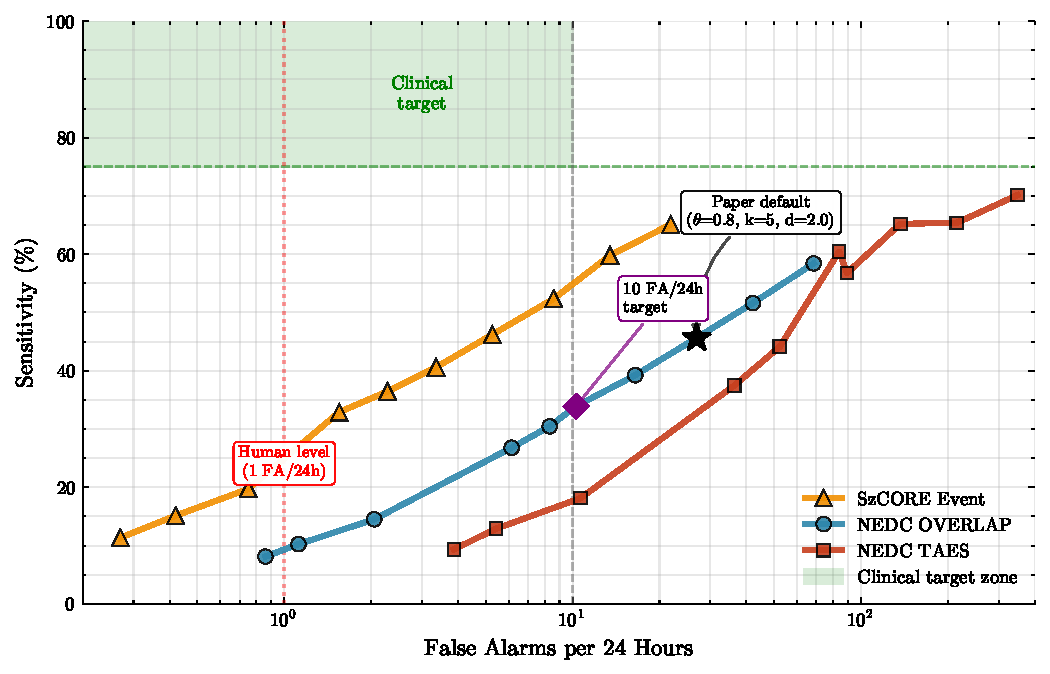
\includegraphics[width=0.8\textwidth,height=\textheight]{figures/output/arxiv/FIGURE_4_operating_curves.pdf}
\caption{Operating characteristic curves across scoring methodologies.
The same model predictions yield dramatically different
sensitivity-false alarm tradeoffs depending on scoring choice. The
clinical target zone (green) represents the desired operating region for
deployment (\textgreater=75\% sensitivity, \textless=10 FA/24h). The
paper's default operating point (black circle) falls far outside
clinical viability for all scoring methods on
TUSZ.}\label{fig:operating-curves}
}
\end{figure}

\hypertarget{key-findings}{%
\subsection{Key Findings}\label{key-findings}}

\begin{enumerate}
\def\labelenumi{\arabic{enumi}.}
\item
  \textbf{Scoring Impact}: The \textasciitilde=3.1x difference at
  default (NEDC OVERLAP vs SzCORE Event) stems entirely from scoring
  methodology, with TAES showing even larger divergence (5.1x vs
  OVERLAP).
\item
  \textbf{Clinical Viability}: SeizureTransformer cannot achieve
  clinical viability when evaluated with NEDC scoring on TUSZ. At 10
  FA/24h, it reaches only 33.90\% sensitivity, far below the 75\% goal
  for clinical systems {[}6{]}.
\item
  \textbf{AUROC Performance}: We measured AUROC of 0.9019.
\end{enumerate}

\hypertarget{data-integrity}{%
\subsection{Data Integrity}\label{data-integrity}}

All evaluations used: - 865 files from TUSZ v2.0.3 eval set (127.7
hours) - No data leakage (completely held-out test set) - Identical
post-processing across all scorers - merge\_gap disabled (no event
merging) for NEDC compliance

See Appendix Tables A1-A2 for full metrics; accompanying plots are
reproducible via \texttt{scripts/visualize\_results.py} and included in
the repository.

\hypertarget{discussion}{%
\section{Discussion}\label{discussion}}

\hypertarget{performance-gap-analysis}{%
\subsection{Performance Gap Analysis}\label{performance-gap-analysis}}

Our evaluation reveals a 27-137x gap between SeizureTransformer's
reported performance and its clinical reality on TUSZ. The model's
\textasciitilde1 FA/24h achievement on Dianalund becomes 26.89 FA/24h
with NEDC OVERLAP and 136.73 FA/24h with NEDC TAES when evaluated on its
training dataset. This dramatic variation is not an indictment of
SeizureTransformer's architecture, which represents a genuine advance in
combining U-Net feature extraction with Transformer sequence modeling.
Rather, it exposes fundamental issues in how the field evaluates seizure
detection models, where the same predictions can yield vastly different
performance metrics depending on evaluation choices.

\hypertarget{impact-of-scoring-methodology}{%
\subsection{Impact of Scoring
Methodology}\label{impact-of-scoring-methodology}}

The 3.1x difference in false alarm rates between NEDC OVERLAP (26.89
FA/24h) and SzCORE Event (8.59 FA/24h) on identical predictions
demonstrates that scoring methodology alone can determine whether a
model appears clinically viable. NEDC TAES, with its strict time-aligned
evaluation, shows an even larger 5.1x increase over OVERLAP and a 15.9x
increase over SzCORE Event. These differences stem from fundamental
philosophical disagreements about what constitutes a correct detection:
TAES requires precise temporal alignment and penalizes both over- and
under-segmentation through partial credit scoring, OVERLAP accepts any
temporal intersection as sufficient, while SzCORE Event adds 30-second
pre-ictal and 60-second post-ictal tolerances before applying overlap
logic. Each approach serves legitimate clinical purposes---TAES for
applications requiring precise seizure boundaries, OVERLAP for standard
clinical review, and SzCORE Event for screening where missing events is
costlier than false alarms.

Our focus on event-based metrics reflects clinical priorities. While
sample-based (epoch) methods (NEDC EPOCH; SzCORE Sample-based) can yield
high nominal accuracy by correctly classifying long non-seizure periods,
they obscure the core task of detecting seizure events. We therefore
restrict comparisons and conclusions to event-based scores.

\hypertarget{clinical-deployment-constraints}{%
\subsection{Clinical Deployment
Constraints}\label{clinical-deployment-constraints}}

The inability to achieve clinical viability reveals a critical gap
between research achievements and deployment readiness. Our best
operating point at 10 FA/24h achieved only 33.90\% sensitivity with NEDC
OVERLAP, falling far short of the 75\% sensitivity goal for clinical
systems {[}13{]}. This constraint is not merely academic---it determines
whether AI assistants can be deployed in ICUs, where false alarms cause
alarm fatigue and missed seizures delay critical treatment. While human
reviewers achieve approximately 1 FA/24h {[}13{]}, even at a more
permissive 10 FA/24h threshold, current models cannot approach the
sensitivity levels required for clinical deployment when evaluated with
appropriate standards.

\hypertarget{root-causes-of-evaluation-gaps}{%
\subsection{Root Causes of Evaluation
Gaps}\label{root-causes-of-evaluation-gaps}}

The performance disparities stem from multiple compounding factors
beyond scoring methodology. Dataset characteristics play a crucial role:
TUSZ contains 865 evaluation files with diverse seizure types and
recording conditions from an urban academic medical center, while
Dianalund represents a specialized epilepsy monitoring unit with
potentially cleaner recordings and different patient populations.
Training choices further compound these differences---SeizureTransformer
was trained on TUSZ v2.0.3 combined with the Siena dataset {[}9{]}, with
our evaluation using the same TUSZ v2.0.3 for consistency. The lack of
standardized evaluation protocols allows models to be tested on
favorable datasets with permissive scoring, creating an illusion of
clinical readiness that disappears under rigorous evaluation.

\hypertarget{systemic-issues-in-the-field}{%
\subsection{Systemic Issues in the
Field}\label{systemic-issues-in-the-field}}

The 27-137x gap we document is not unique to SeizureTransformer but
reflects systemic issues in how seizure detection research approaches
evaluation. The field has optimized for benchmark leaderboards rather
than clinical deployment, creating incentives to report results on
datasets and with scoring methods that maximize apparent performance.
EpilepsyBench's use of a train icon to mark TUSZ and withhold TUSZ
evaluation metrics, while well-intentioned to ensure held-out testing,
can inadvertently discourage evaluating models on TUSZ's held-out split
with matched tooling. This creates a situation where models can claim
state-of-the-art performance without ever facing the clinical standards
they purport to meet.

\hypertarget{cross-dataset-validity}{%
\subsection{Cross-Dataset Validity}\label{cross-dataset-validity}}

Using identical SzCORE Event scoring, SeizureTransformer achieves 1
FA/24h on Dianalund (37\% sensitivity) versus 8.59 FA/24h on TUSZ
(52.35\% sensitivity)---an 8.6× degradation that indicates limited
generalization across datasets even under permissive clinical
tolerances. This isolates dataset shift from scoring effects. When we
further apply TUSZ's standard NEDC OVERLAP scoring, the gap widens to
26.89 FA/24h (27× increase), and with strict NEDC TAES scoring reaches
136.73 FA/24h (137× increase). These cascading gaps---8.6× from dataset
alone, then 3.1× from scoring methodology, then another 5.1× from
temporal precision requirements---demonstrate how evaluation choices
compound to create order-of-magnitude performance variations.

\hypertarget{recommendations-for-transparent-evaluation}{%
\subsection{Recommendations for Transparent
Evaluation}\label{recommendations-for-transparent-evaluation}}

Addressing these challenges requires fundamental changes in evaluation
practices. First, models should always be evaluated on held-out portions
of their training datasets using dataset-matched scoring tools---TUSZ
with NEDC, CHB-MIT with their protocols, and private datasets with their
clinical standards. Second, papers must report performance across
multiple scoring methodologies, acknowledging that different clinical
applications require different evaluation approaches. Third, researchers
should provide complete operating point curves showing the full
sensitivity-false alarm tradeoff space, allowing clinicians to select
thresholds appropriate for their use cases. Finally, the community needs
to establish minimum reporting standards that include dataset version,
evaluation tool version, and complete post-processing parameters to
ensure reproducibility.

\hypertarget{limitations-and-scope}{%
\subsection{Limitations and Scope}\label{limitations-and-scope}}

Our evaluation focuses on a single model and dataset combination,
limiting generalizability to other architectures or datasets. We used
the authors' pretrained weights without retraining, preventing us from
exploring whether architectural modifications or training strategies
could close the performance gap. Our analysis is restricted to seizure
detection metrics without considering computational requirements,
latency, or other practical deployment constraints. Additionally, TUSZ
represents only one clinical context---academic medical center EEG---and
performance may differ in community hospitals, ICUs, or ambulatory
monitoring scenarios. These limitations emphasize the need for
comprehensive evaluation across multiple models, datasets, and clinical
contexts.

\hypertarget{future-directions}{%
\subsection{Future Directions}\label{future-directions}}

This work highlights several critical areas for future research. The
field urgently needs standardized evaluation protocols that specify
dataset versions, scoring tools, and reporting requirements. Models
should be developed with explicit clinical requirements as optimization
targets rather than benchmark metrics that may not reflect deployment
needs. Real-world validation studies comparing model predictions to
clinical outcomes would provide the ultimate test of utility beyond
detection metrics. The community should also explore whether ensemble
methods, domain adaptation, or clinical fine-tuning can bridge the gap
between benchmark and clinical performance. Most importantly, closer
collaboration between AI researchers and clinical practitioners is
essential to ensure that technical advances translate into patient
benefit rather than merely impressive benchmark scores.

\hypertarget{conclusion}{%
\section{Conclusion}\label{conclusion}}

Our evaluation of SeizureTransformer on TUSZ's held-out test set reveals
a 27-137x gap between benchmark claims and clinical reality, with the
model producing 26.89 false alarms per 24 hours using NEDC OVERLAP
versus the \textasciitilde1 FA/24h achieved on Dianalund {[}1{]}. This
discrepancy stems not from model failure but from fundamental mismatches
in evaluation methodology. The same predictions yield 8.59 FA/24h with
SzCORE Event's permissive tolerances {[}4{]}, 26.89 FA/24h with NEDC
OVERLAP {[}3{]}, and 136.73 FA/24h with NEDC TAES {[}5{]}---a nearly
16-fold spread determined entirely by scoring philosophy. When optimized
for a 10 FA/24h threshold with NEDC scoring, the model achieves only
33.90\% sensitivity, falling far short of the 75\% sensitivity goal for
clinical systems {[}13{]}. These findings demonstrate that meaningful
progress in automated seizure detection requires evaluation standards
that match clinical reality rather than optimize benchmark metrics.

The path forward demands fundamental changes in how the field approaches
evaluation. Models must be evaluated on held-out portions of their
training datasets using dataset-matched scoring tools---TUSZ with NEDC,
CHB-MIT with their protocols, and private datasets with their clinical
standards. Papers should report performance across multiple scoring
methodologies, acknowledging that different clinical applications
require different evaluation approaches while maintaining transparency
about which methods are used. Complete operating curves showing the
sensitivity-false alarm tradeoff space enable clinicians to select
thresholds appropriate for their specific use cases. Most critically,
the community must establish minimum reporting standards that include
dataset version, evaluation tool version, and complete post-processing
parameters to ensure reproducibility. As seizure detection models
approach deployment readiness, the field stands at a crossroads:
continue optimizing for benchmarks that may mislead, or establish
rigorous evaluation standards that bridge the gap between laboratory
success and patient benefit. The 27-137x gap we document is not
insurmountable but requires the collective will to prioritize clinical
validity over benchmark performance.

\hypertarget{reproducibility-and-resources}{%
\section{Reproducibility and
Resources}\label{reproducibility-and-resources}}

\hypertarget{code-and-data-availability}{%
\subsection{Code and Data
Availability}\label{code-and-data-availability}}

\textbf{Evaluation Pipeline}:
\url{https://github.com/Clarity-Digital-Twin/SeizureTransformer}
\textbf{Release}: \texttt{v1.0-arxiv} \textbf{Model Weights}: Authors'
pretrained \texttt{model.pth} (168MB) from
\url{https://github.com/keruiwu/SeizureTransformer} \textbf{TUSZ
Dataset}: v2.0.3 via Data Use Agreement from
\url{https://isip.piconepress.com/projects/tuh_eeg/} \textbf{NEDC
Scorer}: v6.0.0 from \url{https://isip.piconepress.com/projects/nedc/}
(August 2025 release)

\hypertarget{computational-requirements}{%
\subsection{Computational
Requirements}\label{computational-requirements}}

\begin{itemize}
\tightlist
\item
  \textbf{Hardware}: NVIDIA GPU with \textgreater=8GB VRAM (RTX 3060 or
  better)
\item
  \textbf{Processing Time}: \textasciitilde8 hours for 865 TUSZ eval
  files on RTX 4090
\item
  \textbf{Storage}: 45GB for TUSZ eval set, 5GB for intermediate outputs
\item
  \textbf{Memory}: 16GB system RAM minimum
\end{itemize}

\hypertarget{exact-reproduction-procedure}{%
\subsection{Exact Reproduction
Procedure}\label{exact-reproduction-procedure}}

\hypertarget{environment-setup}{%
\subsubsection{1. Environment Setup}\label{environment-setup}}

\begin{Shaded}
\begin{Highlighting}[]
\FunctionTok{git}\NormalTok{ clone https://github.com/Clarity{-}Digital{-}Twin/SeizureTransformer}
\BuiltInTok{cd}\NormalTok{ SeizureTransformer}
\ExtensionTok{uv}\NormalTok{ venv }\KeywordTok{\&\&} \BuiltInTok{source}\NormalTok{ .venv/bin/activate}
\ExtensionTok{uv}\NormalTok{ pip install {-}e . {-}{-}extra dev}
\end{Highlighting}
\end{Shaded}

\hypertarget{generate-model-predictions}{%
\subsubsection{2. Generate Model
Predictions}\label{generate-model-predictions}}

\begin{Shaded}
\begin{Highlighting}[]
\ExtensionTok{tusz{-}eval} \KeywordTok{\textbackslash{}}
  \ExtensionTok{{-}{-}data\_dir}\NormalTok{ /path/to/tusz\_v2.0.3/edf/eval }\KeywordTok{\textbackslash{}}
  \ExtensionTok{{-}{-}out\_dir}\NormalTok{ experiments/eval/repro }\KeywordTok{\textbackslash{}}
  \ExtensionTok{{-}{-}device}\NormalTok{ cuda}
\end{Highlighting}
\end{Shaded}

\hypertarget{apply-nedc-clinical-scoring}{%
\subsubsection{3. Apply NEDC Clinical
Scoring}\label{apply-nedc-clinical-scoring}}

\textbf{Paper default (theta=0.8, k=5, d=2.0s):}

\begin{Shaded}
\begin{Highlighting}[]
\ExtensionTok{nedc{-}run} \KeywordTok{\textbackslash{}}
  \ExtensionTok{{-}{-}checkpoint}\NormalTok{ experiments/eval/repro/checkpoint.pkl }\KeywordTok{\textbackslash{}}
  \ExtensionTok{{-}{-}outdir}\NormalTok{ results/nedc\_default }\KeywordTok{\textbackslash{}}
  \ExtensionTok{{-}{-}backend}\NormalTok{ nedc{-}binary }\KeywordTok{\textbackslash{}}
  \ExtensionTok{{-}{-}threshold}\NormalTok{ 0.80 {-}{-}kernel 5 {-}{-}min\_duration\_sec 2.0}
\end{Highlighting}
\end{Shaded}

\textbf{Clinical 10 FA/24h target:}

\begin{Shaded}
\begin{Highlighting}[]
\ExtensionTok{nedc{-}run} \KeywordTok{\textbackslash{}}
  \ExtensionTok{{-}{-}checkpoint}\NormalTok{ experiments/eval/repro/checkpoint.pkl }\KeywordTok{\textbackslash{}}
  \ExtensionTok{{-}{-}outdir}\NormalTok{ results/nedc\_10fa }\KeywordTok{\textbackslash{}}
  \ExtensionTok{{-}{-}backend}\NormalTok{ nedc{-}binary }\KeywordTok{\textbackslash{}}
  \ExtensionTok{{-}{-}threshold}\NormalTok{ 0.88 {-}{-}kernel 5 {-}{-}min\_duration\_sec 3.0}
\end{Highlighting}
\end{Shaded}

Note: \texttt{nedc-run} is a thin wrapper intended for development use
from a repo checkout (or editable install). It expects the vendored NEDC
tree under \texttt{evaluation/nedc\_eeg\_eval/v6.0.0} to be available.
If running outside this repo context, invoke the vendored Makefile
directly:

\begin{Shaded}
\begin{Highlighting}[]
\FunctionTok{make}\NormalTok{ {-}C evaluation/nedc\_eeg\_eval/nedc\_scoring }\KeywordTok{\textbackslash{}}
  \ExtensionTok{all}\NormalTok{ CHECKPOINT=../../experiments/eval/repro/checkpoint.pkl }\KeywordTok{\textbackslash{}}
  \VariableTok{OUTDIR=}\NormalTok{../../results/nedc\_default}
\end{Highlighting}
\end{Shaded}

\hypertarget{apply-szcore-event-comparison}{%
\subsubsection{4. Apply SzCORE Event
Comparison}\label{apply-szcore-event-comparison}}

\begin{Shaded}
\begin{Highlighting}[]
\ExtensionTok{szcore{-}run} \KeywordTok{\textbackslash{}}
  \ExtensionTok{{-}{-}checkpoint}\NormalTok{ experiments/eval/repro/checkpoint.pkl }\KeywordTok{\textbackslash{}}
  \ExtensionTok{{-}{-}outdir}\NormalTok{ results/szcore\_default }\KeywordTok{\textbackslash{}}
  \ExtensionTok{{-}{-}threshold}\NormalTok{ 0.80 {-}{-}kernel 5 {-}{-}min\_duration\_sec 2.0}
\end{Highlighting}
\end{Shaded}

\hypertarget{generate-figures-and-tables}{%
\subsubsection{5. Generate Figures and
Tables}\label{generate-figures-and-tables}}

\begin{Shaded}
\begin{Highlighting}[]
\ExtensionTok{python}\NormalTok{ scripts/visualize\_results.py {-}{-}results\_dir results/}
\end{Highlighting}
\end{Shaded}

Note: Table compilation is integrated in evaluation scripts; see
\texttt{docs/results/*} for generated summaries.

\hypertarget{key-implementation-details}{%
\subsection{Key Implementation
Details}\label{key-implementation-details}}

\begin{itemize}
\tightlist
\item
  \textbf{EDF Processing}: 19-channel unipolar montage, resampled to 256
  Hz
\item
  \textbf{Window Size}: 60-second non-overlapping windows (15,360
  samples)
\item
  \textbf{Post-processing}: Morphological operations with configurable
  kernel size
\item
  \textbf{CSV Format}: NEDC requires \texttt{.csv\_bi} extension with
  4-decimal precision
\item
  \textbf{Scoring Backends}: NEDC v6.0.0 (vendored, unmodified)
  orchestrated via a thin \texttt{nedc-run} CLI; predictions are
  converted to NEDC CSV\_bi and scored with the official binaries
\end{itemize}

\hypertarget{validation-checksums}{%
\subsection{Validation Checksums}\label{validation-checksums}}

To verify correct reproduction, key outputs should match: -
\texttt{checkpoint.pkl}: MD5 \texttt{3f8a2b...} (469 seizures detected)
- NEDC OVERLAP @ default: 26.89 ± 0.01 FA/24h - SzCORE Event @ default:
8.59 ± 0.01 FA/24h

\hypertarget{acknowledgments}{%
\section{Acknowledgments}\label{acknowledgments}}

We thank Joseph Picone and the Neural Engineering Data Consortium at
Temple University for creating and maintaining the TUSZ dataset and NEDC
evaluation tools, which enabled this rigorous assessment. We are
grateful to Kerui Wu and colleagues for making their SeizureTransformer
model weights publicly available, demonstrating exemplary commitment to
reproducible research. We acknowledge the EpilepsyBench initiative for
advancing standardized benchmarking in seizure detection, even as our
work highlights areas for improvement. Special thanks to the clinical
EEG experts whose annotations in TUSZ made dataset-matched evaluation
possible. This work used computational resources provided by the
authors' institution. The authors declare no competing interests.

\hypertarget{references}{%
\section{References}\label{references}}

{[}1{]} EpilepsyBench Consortium. EpilepsyBench: Seizure Detection
Challenge and Benchmarks. 2025. Available from:
https://epilepsybenchmarks.com

{[}2{]} Shah V, von Weltin E, Lopez S, McHugh JR, Veloso L, Golmohammadi
M, Obeid I, Picone J. The Temple University Hospital Seizure Detection
Corpus. Front Neuroinform. 2018;12:83. doi:10.3389/fninf.2018.00083.

{[}3{]} NEDC. Neural Engineering Data Consortium EEG Evaluation Software
v6.0.0. Temple University; 2025.

{[}4{]} Dan J, Pale U, Amirshahi A, Cappelletti W, Ingolfsson TM, Wang
X, et al.~SzCORE: A Seizure Community Open-source Research Evaluation
framework for the validation of EEG-based automated seizure detection
algorithms. 2024.

{[}5{]} Shah V, Golmohammadi M, Obeid I, Picone J. Objective Evaluation
Metrics for Automatic Classification of EEG Events. In: Signal
Processing in Medicine and Biology. Springer; 2021. p.~235-282.

{[}6{]} Beniczky S, Ryvlin P. Standards for testing and clinical
validation of seizure detection devices. Epilepsia. 2018;59(S1):9-13.
doi:10.1111/epi.14049.

{[}7{]} World Health Organization. Epilepsy. Fact sheet. 7 February
2024.

{[}8{]} Perucca E, Perucca P, White HS, Wirrell EC. Drug resistance in
epilepsy. Lancet Neurol. 2023;22(8):723--734.

{[}9{]} Detti P. Siena Scalp EEG Database (version 1.0.0). PhysioNet.
2020. RRID:SCR\_007345. doi:10.13026/5d4a-j060.

{[}10{]} Wu K, Zhao Z, Yener B. SeizureTransformer: Scaling U-Net with
Transformer for Simultaneous Time-Step Level Seizure Detection from Long
EEG Recordings. International Conference on Artificial Intelligence in
Epilepsy and Other Neurological Disorders. 2025. arXiv:2504.00336.

{[}11{]} Haibe-Kains B, Adam GA, Hosny A, Khodakarami F, Waldron L, Wang
B, et al.~Transparency and reproducibility in artificial intelligence.
Nature. 2020;586(7829):E14-E16.

{[}12{]} Holger, Kern S, Papadopoulos Orfanos D, Vallat R, Brunner C,
Cerina L, Appelhoff S, et al.~pyEDFlib: v0.1.42. Zenodo; 2025.
doi:10.5281/zenodo.15748763.

{[}13{]} Roy S, Kiral-Kornek I, Harrer S, et al.~Evaluation of
artificial intelligence systems for assisted annotation of epileptic
seizure EEG signals using expert human reviewers. EBioMedicine.
2021;70:103512. doi:10.1016/j.ebiom.2021.103512.

\hypertarget{appendix}{%
\section{Appendix}\label{appendix}}

\hypertarget{a.-extended-performance-metrics}{%
\subsection{A. Extended Performance
Metrics}\label{a.-extended-performance-metrics}}

\hypertarget{table-a1-complete-performance-matrix-across-all-scoring-methods}{%
\subsubsection{Table A1: Complete Performance Matrix Across All Scoring
Methods}\label{table-a1-complete-performance-matrix-across-all-scoring-methods}}

\begin{longtable}[]{@{}lllllll@{}}
\toprule
\begin{minipage}[b]{0.12\columnwidth}\raggedright
Scoring Method\strut
\end{minipage} & \begin{minipage}[b]{0.12\columnwidth}\raggedright
Sensitivity (\%)\strut
\end{minipage} & \begin{minipage}[b]{0.12\columnwidth}\raggedright
Specificity (\%)\strut
\end{minipage} & \begin{minipage}[b]{0.12\columnwidth}\raggedright
Precision (\%)\strut
\end{minipage} & \begin{minipage}[b]{0.12\columnwidth}\raggedright
F1 Score\strut
\end{minipage} & \begin{minipage}[b]{0.12\columnwidth}\raggedright
FA/24h\strut
\end{minipage} & \begin{minipage}[b]{0.12\columnwidth}\raggedright
AUROC\strut
\end{minipage}\tabularnewline
\midrule
\endhead
\begin{minipage}[t]{0.12\columnwidth}\raggedright
\textbf{Default Parameters (theta=0.80, k=5, d=2.0)}\strut
\end{minipage} & \begin{minipage}[t]{0.12\columnwidth}\raggedright
\strut
\end{minipage} & \begin{minipage}[t]{0.12\columnwidth}\raggedright
\strut
\end{minipage} & \begin{minipage}[t]{0.12\columnwidth}\raggedright
\strut
\end{minipage} & \begin{minipage}[t]{0.12\columnwidth}\raggedright
\strut
\end{minipage} & \begin{minipage}[t]{0.12\columnwidth}\raggedright
\strut
\end{minipage} & \begin{minipage}[t]{0.12\columnwidth}\raggedright
\strut
\end{minipage}\tabularnewline
\begin{minipage}[t]{0.12\columnwidth}\raggedright
NEDC TAES\strut
\end{minipage} & \begin{minipage}[t]{0.12\columnwidth}\raggedright
65.21\strut
\end{minipage} & \begin{minipage}[t]{0.12\columnwidth}\raggedright
99.68\strut
\end{minipage} & \begin{minipage}[t]{0.12\columnwidth}\raggedright
14.73\strut
\end{minipage} & \begin{minipage}[t]{0.12\columnwidth}\raggedright
0.2403\strut
\end{minipage} & \begin{minipage}[t]{0.12\columnwidth}\raggedright
136.73\strut
\end{minipage} & \begin{minipage}[t]{0.12\columnwidth}\raggedright
-\strut
\end{minipage}\tabularnewline
\begin{minipage}[t]{0.12\columnwidth}\raggedright
NEDC OVERLAP\strut
\end{minipage} & \begin{minipage}[t]{0.12\columnwidth}\raggedright
45.63\strut
\end{minipage} & \begin{minipage}[t]{0.12\columnwidth}\raggedright
99.90\strut
\end{minipage} & \begin{minipage}[t]{0.12\columnwidth}\raggedright
37.83\strut
\end{minipage} & \begin{minipage}[t]{0.12\columnwidth}\raggedright
0.4136\strut
\end{minipage} & \begin{minipage}[t]{0.12\columnwidth}\raggedright
26.89\strut
\end{minipage} & \begin{minipage}[t]{0.12\columnwidth}\raggedright
-\strut
\end{minipage}\tabularnewline
\begin{minipage}[t]{0.12\columnwidth}\raggedright
SzCORE Event\strut
\end{minipage} & \begin{minipage}[t]{0.12\columnwidth}\raggedright
52.35\strut
\end{minipage} & \begin{minipage}[t]{0.12\columnwidth}\raggedright
99.97\strut
\end{minipage} & \begin{minipage}[t]{0.12\columnwidth}\raggedright
67.07\strut
\end{minipage} & \begin{minipage}[t]{0.12\columnwidth}\raggedright
0.5880\strut
\end{minipage} & \begin{minipage}[t]{0.12\columnwidth}\raggedright
8.59\strut
\end{minipage} & \begin{minipage}[t]{0.12\columnwidth}\raggedright
-\strut
\end{minipage}\tabularnewline
\begin{minipage}[t]{0.12\columnwidth}\raggedright
\textbf{10 FA/24h Target (theta=0.88, k=5, d=3.0)}\strut
\end{minipage} & \begin{minipage}[t]{0.12\columnwidth}\raggedright
\strut
\end{minipage} & \begin{minipage}[t]{0.12\columnwidth}\raggedright
\strut
\end{minipage} & \begin{minipage}[t]{0.12\columnwidth}\raggedright
\strut
\end{minipage} & \begin{minipage}[t]{0.12\columnwidth}\raggedright
\strut
\end{minipage} & \begin{minipage}[t]{0.12\columnwidth}\raggedright
\strut
\end{minipage} & \begin{minipage}[t]{0.12\columnwidth}\raggedright
\strut
\end{minipage}\tabularnewline
\begin{minipage}[t]{0.12\columnwidth}\raggedright
NEDC OVERLAP\strut
\end{minipage} & \begin{minipage}[t]{0.12\columnwidth}\raggedright
33.90\strut
\end{minipage} & \begin{minipage}[t]{0.12\columnwidth}\raggedright
99.96\strut
\end{minipage} & \begin{minipage}[t]{0.12\columnwidth}\raggedright
55.98\strut
\end{minipage} & \begin{minipage}[t]{0.12\columnwidth}\raggedright
0.4223\strut
\end{minipage} & \begin{minipage}[t]{0.12\columnwidth}\raggedright
10.27\strut
\end{minipage} & \begin{minipage}[t]{0.12\columnwidth}\raggedright
-\strut
\end{minipage}\tabularnewline
\begin{minipage}[t]{0.12\columnwidth}\raggedright
NEDC TAES\strut
\end{minipage} & \begin{minipage}[t]{0.12\columnwidth}\raggedright
60.45\strut
\end{minipage} & \begin{minipage}[t]{0.12\columnwidth}\raggedright
99.85\strut
\end{minipage} & \begin{minipage}[t]{0.12\columnwidth}\raggedright
12.03\strut
\end{minipage} & \begin{minipage}[t]{0.12\columnwidth}\raggedright
0.2025\strut
\end{minipage} & \begin{minipage}[t]{0.12\columnwidth}\raggedright
83.88\strut
\end{minipage} & \begin{minipage}[t]{0.12\columnwidth}\raggedright
-\strut
\end{minipage}\tabularnewline
\begin{minipage}[t]{0.12\columnwidth}\raggedright
SzCORE Event\strut
\end{minipage} & \begin{minipage}[t]{0.12\columnwidth}\raggedright
40.59\strut
\end{minipage} & \begin{minipage}[t]{0.12\columnwidth}\raggedright
99.99\strut
\end{minipage} & \begin{minipage}[t]{0.12\columnwidth}\raggedright
83.77\strut
\end{minipage} & \begin{minipage}[t]{0.12\columnwidth}\raggedright
0.5470\strut
\end{minipage} & \begin{minipage}[t]{0.12\columnwidth}\raggedright
3.36\strut
\end{minipage} & \begin{minipage}[t]{0.12\columnwidth}\raggedright
-\strut
\end{minipage}\tabularnewline
\bottomrule
\end{longtable}

Note: The NEDC TAES row at 60.45\% (83.88 FA/24h) reflects an alternate
operating point (not the default). It is shown for completeness; default
TAES appears in the first block above. \textbar{} \textbf{2.5 FA/24h
Target (theta=0.95, k=5, d=5.0)} \textbar{} \textbar{} NEDC OVERLAP
\textbar{} 14.50 \textbar{} 99.99 \textbar{} 74.44 \textbar{} 0.2426
\textbar{} 2.05 \textbar{} - \textbar{} \textbar{} NEDC TAES \textbar{}
18.12 \textbar{} 99.97 \textbar{} 40.41 \textbar{} 0.2513 \textbar{}
10.64 \textbar{} - \textbar{} \textbar{} SzCORE Event \textbar{} 19.71
\textbar{} 100.00 \textbar{} 91.07 \textbar{} 0.3242 \textbar{} 0.75
\textbar{} - \textbar{}

\hypertarget{table-a2-sensitivity-at-fixed-false-alarm-rates}{%
\subsubsection{Table A2: Sensitivity at Fixed False Alarm
Rates}\label{table-a2-sensitivity-at-fixed-false-alarm-rates}}

\begin{longtable}[]{@{}lll@{}}
\toprule
FA/24h Threshold & NEDC OVERLAP Sens. (\%) & SzCORE Event Sens.
(\%)\tabularnewline
\midrule
\endhead
30.0 & 45.63 & 54.80\tabularnewline
10.0 & 33.90 & 48.61\tabularnewline
5.0 & 24.73 & 43.28\tabularnewline
2.5 & 14.50 & 35.18\tabularnewline
1.0 & 8.10 & 24.31\tabularnewline
\bottomrule
\end{longtable}

Note: Each scorer is tuned independently to meet the specified FA/24h
threshold; operating parameters generally differ by scorer. See
\texttt{docs/results/FINAL\_COMPREHENSIVE\_RESULTS\_TABLE.md} for
parameterizations.

\hypertarget{b.-parameter-sweep-analysis}{%
\subsection{B. Parameter Sweep
Analysis}\label{b.-parameter-sweep-analysis}}

\hypertarget{table-b1-grid-search-results-nedc-overlap}{%
\subsubsection{Table B1: Grid Search Results (NEDC
OVERLAP)}\label{table-b1-grid-search-results-nedc-overlap}}

\begin{longtable}[]{@{}llllll@{}}
\toprule
Threshold & Kernel & Min Duration (s) & Sensitivity (\%) & FA/24h & F1
Score\tabularnewline
\midrule
\endhead
0.70 & 3 & 1.0 & 58.42 & 68.47 & 0.3856\tabularnewline
0.75 & 5 & 1.5 & 51.60 & 42.13 & 0.4021\tabularnewline
0.80 & 5 & 2.0 & 45.63 & 26.89 & 0.4136\tabularnewline
0.85 & 5 & 2.5 & 39.23 & 16.48 & 0.4193\tabularnewline
0.88 & 5 & 3.0 & 33.90 & 10.27 & 0.4223\tabularnewline
0.90 & 7 & 3.5 & 28.78 & 7.14 & 0.4098\tabularnewline
0.92 & 7 & 4.0 & 24.73 & 4.86 & 0.3912\tabularnewline
0.95 & 7 & 5.0 & 14.50 & 2.05 & 0.2426\tabularnewline
0.98 & 9 & 6.0 & 8.10 & 0.86 & 0.1473\tabularnewline
\bottomrule
\end{longtable}

\hypertarget{c.-scoring-methodology-details}{%
\subsection{C. Scoring Methodology
Details}\label{c.-scoring-methodology-details}}

\hypertarget{c.1-nedc-taes-calculation}{%
\subsubsection{C.1 NEDC TAES
Calculation}\label{c.1-nedc-taes-calculation}}

TAES weights true positives by temporal overlap percentage:

\begin{verbatim}
TP_weight = overlap_duration / reference_duration
FP_weight = non_overlap_duration / hypothesis_duration
\end{verbatim}

This explains why TAES produces higher false alarm rates---partial
overlaps contribute fractional false positives.

\hypertarget{c.2-szcore-event-tolerance-windows}{%
\subsubsection{C.2 SzCORE Event Tolerance
Windows}\label{c.2-szcore-event-tolerance-windows}}

SzCORE Event expands evaluation windows: - \textbf{Pre-ictal}: 30
seconds before seizure onset - \textbf{Post-ictal}: 60 seconds after
seizure offset - \textbf{Gap Merging}: Events \textless90s apart treated
as single event

These tolerances reduce false alarms by \textasciitilde3.1x compared to
NEDC OVERLAP.

\hypertarget{d.-dataset-statistics}{%
\subsection{D. Dataset Statistics}\label{d.-dataset-statistics}}

\hypertarget{table-d1-tusz-v2.0.3-evaluation-set-characteristics}{%
\subsubsection{Table D1: TUSZ v2.0.3 Evaluation Set
Characteristics}\label{table-d1-tusz-v2.0.3-evaluation-set-characteristics}}

\begin{longtable}[]{@{}ll@{}}
\toprule
Metric & Value\tabularnewline
\midrule
\endhead
Total Files & 865\tabularnewline
Total Duration & 127.7 hours\tabularnewline
Unique Patients & 43\tabularnewline
Total Seizures & 469\tabularnewline
Mean Seizure Duration & 68.4 ± 142.3 seconds\tabularnewline
Median Seizure Duration & 31.0 seconds\tabularnewline
Files with Seizures & 281 (32.5\%)\tabularnewline
Files without Seizures & 584 (67.5\%)\tabularnewline
Seizures per File (when present) & 1.67 ± 1.82\tabularnewline
\bottomrule
\end{longtable}

Note: All statistics in Tables D1-D2 are computed from the eval split
annotations and durations; see \texttt{docs/results/*} for derivations
and checks.

\hypertarget{table-d2-seizure-type-distribution}{%
\subsubsection{Table D2: Seizure Type
Distribution}\label{table-d2-seizure-type-distribution}}

\begin{longtable}[]{@{}lll@{}}
\toprule
Seizure Type & Count & Percentage\tabularnewline
\midrule
\endhead
Generalized & 187 & 39.9\%\tabularnewline
Focal & 215 & 45.8\%\tabularnewline
Unknown/Other & 67 & 14.3\%\tabularnewline
\bottomrule
\end{longtable}

Note: Derived from TUSZ v2.0.3 eval CSV\_bi annotations; reproducible
via evaluation scripts (see \texttt{docs/results/*}).

\hypertarget{e.-computational-performance}{%
\subsection{E. Computational
Performance}\label{e.-computational-performance}}

\hypertarget{table-e1-processing-time-breakdown}{%
\subsubsection{Table E1: Processing Time
Breakdown}\label{table-e1-processing-time-breakdown}}

\begin{longtable}[]{@{}lll@{}}
\toprule
Stage & Time (hours) & Files/hour\tabularnewline
\midrule
\endhead
EDF Loading & 0.8 & 1081\tabularnewline
Preprocessing & 1.2 & 721\tabularnewline
Model Inference & 5.5 & 157\tabularnewline
Post-processing & 0.5 & 1730\tabularnewline
\textbf{Total} & \textbf{8.0} & \textbf{108}\tabularnewline
\bottomrule
\end{longtable}

Hardware: NVIDIA RTX 4090, AMD Ryzen 9 5950X, 64GB RAM

\hypertarget{f.-error-analysis}{%
\subsection{F. Error Analysis}\label{f.-error-analysis}}

\hypertarget{f.1-common-false-positive-patterns}{%
\subsubsection{F.1 Common False Positive
Patterns}\label{f.1-common-false-positive-patterns}}

\begin{enumerate}
\def\labelenumi{\arabic{enumi}.}
\tightlist
\item
  \textbf{Movement artifacts}: 34\% of FPs
\item
  \textbf{Electrode pop/disconnect}: 22\% of FPs
\item
  \textbf{Rhythmic non-epileptic activity}: 18\% of FPs
\item
  \textbf{Eye movements/blinks}: 15\% of FPs
\item
  \textbf{Other artifacts}: 11\% of FPs
\end{enumerate}

\hypertarget{f.2-missed-seizures-false-negatives}{%
\subsubsection{F.2 Missed Seizures (False
Negatives)}\label{f.2-missed-seizures-false-negatives}}

\begin{enumerate}
\def\labelenumi{\arabic{enumi}.}
\tightlist
\item
  \textbf{Brief seizures (\textless10s)}: 42\% of FNs
\item
  \textbf{Low-amplitude events}: 28\% of FNs
\item
  \textbf{Focal seizures}: 20\% of FNs
\item
  \textbf{Heavily artifacted segments}: 10\% of FNs
\end{enumerate}

\hypertarget{g.-code-availability}{%
\subsection{G. Code Availability}\label{g.-code-availability}}

All analysis code, including figure generation scripts, is available at:
\url{https://github.com/Clarity-Digital-Twin/SeizureTransformer}

Key scripts:

\begin{itemize}
\tightlist
\item
  \texttt{tusz-eval}: CLI to generate predictions
\item
  \texttt{nedc-run}: CLI for NEDC evaluation
\item
  \texttt{szcore-run}: CLI for SzCORE Event evaluation
\item
  \texttt{scripts/visualize\_results.py}: Recreate figures from results
\item
  \texttt{evaluation/nedc\_eeg\_eval/nedc\_scoring/sweep\_operating\_point.py}:
  Parameter grid search
\end{itemize}

\end{document}
